%%% The ``\documentclass'' command has one parameter, based on the kind of
%%% document you are preparing.
%%%
%%% [annual] - Technical paper accepted for presentation at the ACM SIGGRAPH 
%%%   or SIGGRAPH Asia annual conference.
%%% [sponsored] - Short or full-length technical paper accepted for 
%%%   presentation at an event sponsored by ACM SIGGRAPH
%%%   (but not the annual conference Technical Papers program).
%%% [abstract] - A one-page abstract of your accepted content
%%%   (Technical Sketches, Posters, Emerging Technologies, etc.). 
%%%   Content greater than one page in length should use the "[sponsored]"
%%%   parameter.
%%% [preprint] - A preprint version of your final content.
%%% [review] - A technical paper submitted for review. Includes line
%%%   numbers and anonymization of author and affiliation information.

\documentclass[annual]{acmsiggraph}
\usepackage{algorithm}
\usepackage{algorithmic}
\usepackage{amsmath}
\usepackage{mathtools}
\usepackage{xspace}
\usepackage{array}
\usepackage{epsfig}
\usepackage{subfig}

\usepackage{prog2tex}

\newcommand\CC{\Lang{\mbox{C++}}\xspace}
\newcommand\Lang[1]{\textsc{#1}}
\newcommand{\kw}[1]{\texttt{\textbf{#1}}}
\newcommand{\cd}[1]{\texttt{#1}}

%%% If you are submitting your paper to one of our annual conferences - the 
%%% ACM SIGGRAPH conference held in North America, or the SIGGRAPH Asia 
%%% conference held in Southeast Asia - there are several commands you should 
%%% consider using in the preparation of your document.

%%% 1. ``\TOGonlineID''
%%% When you submit your paper for review, please use the ``\TOGonlineID''
%%% command to include the online ID value assigned to your paper by the
%%% submission management system. Replace '45678' with the value you were
%%% assigned.

\TOGonlineid{45678}

%%% 2. ``\TOGvolume'' and ``\TOGnumber''
%%% If you are preparing a preprint of your accepted paper, and your paper
%%% will be published in an issue of the ACM ``Transactions on Graphics''
%%% journal, replace the ``0'' values in the commands below with the correct
%%% volume and number values for that issue - you'll get them before your
%%% final paper is due.

\TOGvolume{0}
\TOGnumber{0}

%%% 3. ``TOGarticleDOI''
%%% The ``TOGarticleDOI'' command accepts the DOI information provided to you
%%% during production, and which makes up the URLs which identifies the ACM
%%% article page and direct PDF link in the ACM Digital Library.
%%% Replace ``1111111.2222222'' with the values you are given.

\TOGarticleDOI{1111111.2222222}

%%% 4. ``\TOGprojectURL'', ``\TOGvideoURL'', ``\TOGdataURL'', ``\TOGcodeURL''
%%% If you would like to include links to personal repositories for auxiliary
%%% material related your research contribution, you may use one or more of
%%% these commands to define an appropriate URL. The ``\TOGlinkslist'' command
%%% found just before the first section of your document will add hyperlinked
%%% icons to your document, in addition to hyperlinked icons which point to
%%% the ACM Digital Library article page and the ACM Digital Library-held PDF.

\TOGprojectURL{}
\TOGvideoURL{}
\TOGdataURL{}
\TOGcodeURL{}

%%% Replace ``PAPER TEMPLATE TITLE'' with the title of your paper or abstract.

\title{A practical framework for real time ray-tracing of animated skeletal implicit surfaces on the GPU.\\Master Thesis.}
%%% The ``\author{}'' command takes the names and affiliations of each of the
%%% authors of your paper or abstract. The ``\thanks{}'' command takes the
%%% contact information for each author.
%%% For multiple authors, separate each author's information by the ``\and''
%%% command.

\author{Olivier Rouiller\thanks{e-mail: s090842@student.dtu.dk}\\ Department of Informatics and Mathematical Modelling, Danmarks Tekniske Universitet %
 %
}

%%% The ``pdfauthor'' command accepts the authors of the work,
%%% comma-delimited, and adds this information to the PDF metadata.

\pdfauthor{Olivier Rouiller}

%%% Keywords that describe your work. The ``\keywordlist'' command will print
%%% them out.

\keywords{Geometric Modelling, Implicit Surfaces, Real Time Ray-Tracing}

%%% The ``\begin{document}'' command is the start of the document.

%%% If you have user-defined macros, you may include them here.

% example of a user-defined macro called ``remark.''
% \newcommand{\remark}[1]{\textcolor{red}{#1}}

\begin{document}

%%% A ``teaser'' image appears under the title and affiliation information,
%%% horizontally centered, and above the two columns of text. This is OPTIONAL.
%%% If you choose to have a ``teaser'' image, it needs to be placed between
%%% ``\begin{document}'' and ``\maketitle.''

\teaser{



  \includegraphics[width=4.5in]{../../figs/Spider.png}
  \caption{A spider modelled and rendered with our framework.}

%   \includegraphics[height=1.5in]{images/sampleteaser}
%   \caption{Spring Training 2009, Peoria, AZ.}
}

%%% The ``\maketitle'' command must appear after ``\begin{document}'' and,
%%% if you have one, after the definition of your ``teaser'' image, and
%%% before the first ``\section'' command.

\maketitle

%%% Your paper's abstract goes in its own section.

\begin{abstract}


We present a framework consisting of a surface representation based on skeletal implicit surfaces and a ray tracing algorithm that allows to model animated surfaces in real time. This framework allows common effects used in computer graphics such as texturing and displacement mapping and can be to be integrated in a real time renderer. To demonstrate the power of the framework, we build an interactive modelling tool.\\
The surface representation that we use is a subset of skeletal implicit surfaces and we limit ourselves to simple primitives such as points and line segments. We choose degree four polynomials for the convolution kernel. We combine this skeletal representation of the geometry with a hierarchical bone data structure to allow animation.\\
The rendering is done on the GPU in a single pass via ray tracing. The ray-tracing algorithm uses bisection to find the ray-surface intersection and relies on finding points on the ray that are inside the surface.
We propose a method to apply 3D and 2D textures to the model in the fragment shader that is compatible with animation. This method consists in transforming the position of the fragment to it's position in the model's rest pose to compute the texture coordinates with local projectors.

\end{abstract}

%%% ACM Computing Review (CR) categories.
%%% See <http://www.acm.org/class/1998/> for details.
%%% The ``\CRcat'' command takes four arguments.

%%% The ``\keywordlist'' command prints out the keywords.

\keywordlist

%%% The ``\TOGlinkslist'' command will insert hyperlinked icon(s) to your
%%% paper. This includes, at a minimum, hyperlinked icons to the ACM article
%%% page and the ACM Digital Library-held PDF. If you added URLs to
%%% ``\TOGprojectURL'' or the other, similar commands, they will be added to
%%% the list of icons.
%%% Note: this functionality only works for annual-conference papers.


%%% The ``\copyrightspace'' command 
%%% Do not remove this command.

\copyrightspace

%%% This is the first section of the body of your paper.
\begin{figure}[ht]
  \centering
  \includegraphics[width=2.5in]{../../figs/walk.png}
  \caption{A animated alien modelled with skeletal implicit surfaces and ray-traced on the GPU.}
\end{figure}

\section{Introduction}

The usual real time rendering pipeline is based on polygon rasterization. Models are sent to the GPU as lists of indexed polygon as well as other geometric quantities such as normals, texture coordinates, tangent frames and bone transformations in the case of animated models. This way of representing and rendering the geometry is efficient and have proven its usability over years. However, modelling smooth surfaces requires a large number of polygons. Also, polygonal models use a significant memory storage space and sending the polygons to the GPU is a bottleneck on modern architectures.

Other surface representations such as surface patches and implicit surfaces can be used to represent surfaces in a more compact way. These surfaces also allow high level manipulations and can simplify the modelling process. Solutions to render these surfaces exist. The modern graphics pipeline allows to tessellate surface patches on the GPU, thus freeing the bandwidth between the CPU and the GPU. Implicit surfaces can be polygonised and rendered as triangle meshes.

Recently, the increasing power of graphics hardware allowed to render in real time implicit surfaces by ray-tracing on the GPU. This approach allows to benefit from the smoothness of these surfaces. 

We investigate the possibility to use the modelling power of implicit surfaces and the possibilities for ray-tracing implicit surfaces in real time to render animated and textured surfaces based on skeletal implicit surfaces.


\section{Related work}


Implicit surfaces have been used in geometric modelling and procedural geometry modelling because they require few information to represent smooth surfaces of arbitrary topology. 

An implicit surface $S$ is defined as the iso-level set of a scalar field $F$ defined on the 3D space.
$S=\{p \in R^3, F(p)=T\}$ where $T$ has positive value. 

We review some interesting works about modelling with implicit surfaces and about rendering implicit surfaces by ray-tracing.
In the second section of this report we will present our method and how this previous work is interesting for our problem.

\subsection{Geometric modelling with skeletal implicit surfaces}

A skeletal implicit surface is an implicit surface whose potential field is defined by explicit geometric primitives such as points, line segments, polygons or other surfaces. Each of the geometric primitives are independent sources of potential field and the different fields are combined by mathematical operations.
In the most simple case, the potential fields are summed. This produces smooth surfaces that blend together.
In this case the potential field $F$ is the sum of independent functions $F_i$, $F(x) = \displaystyle\sum\limits_{i} F_i(x)$.
Other operations such as difference, minimum or maximum produce more rich surfaces. These operators results in operation on the surface such as intersection, difference and union which are used in Constructive Solid Geometry (CSG). 

\subsubsection{Metaballs}

The most simple kind of implicit surfaces used in computer graphics for modelling is metaballs.
Metaballs were invented by Jim Blin \cite{Blinn1982}, are now very popular in the computer graphics community and are often referred to as Blinn's blobs.
Metaballs are implicit surfaces defined by point primitives. The surface of a single metaball is a sphere and when two metaballs are close enough, they blend into a single smooth surface.

The potential field $F_i$ of a metaball $i$ with center $p_i$ and radius $r_i$ is defined by a decreasing function $f_i$ of the distance to the center of the ball, $F_i(x) = f_i(\|x-p_i\|)$.
The original definition of Blinn's Blobs used an exponential function as the function $f_i$, $f_i(r) = e^{-ar_i}$ where $a$ is a positive scalar.

In practise and for efficiency reasons, we use functions with a similar shape and with compact support. Usually polynomials of degree 4 or 6 are used.
These functions are interesting because they are fast to compute. Also the function vanishes at a certain distance $R$ of the centre of the ball.

Typically the function used are in the form $f(r) = \left(1-\frac{r^2}{R^2}\right)^2$ if $r \leq R$, $0$ otherwise.
The radius $R$ is referred to as effective radius of the metaball.
The sphere centred at the center of the metaball and of radius $R$ is called surface of influence of the metaball.

Metaballs have been mainly used in computer graphics to simulate and render fluids.


\subsubsection{Skeletal implicit surfaces}

Skeletal implicit surfaces are a more general concept than metaballs and are mathematically defined as convolution surfaces.
Modelling with skeletal implicit surfaces have been introduced by Bloomenthal in his doctoral dissertation \cite{Bloomenthal:1996:SDN:238973}.

A convolution surface is defined as an implicit surface with a potential field $f$ defined with explicit primitives and convolution functions.
The field $F$ is of the form $f(x)=g(x)\times h(x)= \displaystyle\int_{R^3} \! g(r)h(x-r) \, \mathrm{d}r $.

$g$ is defined by the explicit geometry. Typically, $g = 1$ on the geometry, $0$ elsewhere. $h$ is the convolution kernel, it is usually a distance function.
With $h$ and $g$ defined in this way, and using point primitives, the integral boils down to the potential field of a metaball.


Convolution surfaces and their applications to computer graphics and geometric modelling have been thoroughly studied by Andrei Sherstyuk in his doctoral dissertation \cite{Sherstyuk}.


\subsubsection{The BlobTree}

Although simple and powerful, skeletal implicit surfaces lack of local control and it is especially hard to create sharp edges and corner using them.

Charles Wyvill addressed this issue by developing a data structure based on skeletal implicit surfaces \cite{Wyvill:98a} and expanding the operation done on the function field to allowing CSG operations. This data structure called the BlobTree as is constructed as a directed acyclic graph where the leaf nodes are geometric primitives and the non-leaf nodes are operation.


\subsubsection{Applications to sketch based modelling}

Finally, recent works on sketched based modelling and high level modelling showed the possibility of building powerful modelling tools based on the BlobTree and allowing intuitive editing of the surface without concern about it's mathematical representation.

Sugihara et. all presented in \cite{Schmidt05shapeshop:sketch-based} a system to edit BlobTree surfaces by sketches and more recently in \cite{SWS10} a system that allows to edit an implicit surface by drawing lines on it and by pushing and pulling them.

Although these works are beyond the scope of our project, they are worth mentioning to show the modelling power of implicit surfaces and to justify their study.

\subsection{Ray tracing implicit surfaces on the GPU}

Rendering implicit surfaces can be done by extracting a polygonal approximation of the surface and rendering the triangle mesh using the usual real time rendering pipeline. The most popular algorithm to polygonize an implicit surface is marching cubes \cite{Lorensen:1987:MCH:37402.37422}.
This algorithm can be optimised to run in real time thus allowing interactive editing and can also be implemented in the GPU \cite{Ryan} for real time rendering of procedural surfaces. However, the output surface requires a large number of polygons in order to produce smooth rendering and it is hard to produce a mesh with polygons that follows the features of the shape.


The other approach to render implicit surfaces is to ray-trace them.
Implicit surfaces are suitable to be ray-traced because of their mathematical representation.
Finding a intersection of a ray with an implicit surface boils down to finding the zeros of the field function along the ray.

With algebraic surfaces, it is possible to compute exactly the intersection by finding the root of an univariate polynomial.

Another approach is to use iterative methods to approximate the root of the function.

\subsubsection{Root finding techniques}

Fukuyama presented in \cite{Fukuyama94amethod} a method to display metaballs by using B\'{e}zier tetrahedra. This method consists in computing the roots of the field function along the ray by solving an univariate polynomial equation.

In \cite{Loop:2006:RGR:1179352.1141939}, Loop et al. presented a method to ray-trace arbitrary algebraic surfaces on the GPU.
With this method it is possible to ray-trace accurately implicit surfaces on the GPU. The method is also based on finding an analytic solution of the polynomial.

 
More recently \cite{Kanamori:2008}, this technique was adapted for metaballs with depth peeling to ray-cast a large number of metaballs at interactive frame rate. The algorithm also use B\'{e}zier clipping as well but evaluates only the metaballs contributing for a pixel by using depth peeling.


\subsubsection{Ray marching and interval arithmetic techniques}

Another way to ray-trace implicit surfaces is to use ray marching techniques.
These techniques consist in finding the ray-surface intersection by evaluating the field function along the ray.

In \cite{Mitchell:1990:RRI:93267.93276}, Mitchell proposed algorithms of interval arithmetic such as bisection to compute efficiently the ray surface intersection with implicit surfaces.   

\subsubsection{Sphere tracing}


Sphere tracing is an adaptive step length search and is known to be efficient to ray-trace surfaces to which we have an evaluation of the distance of a point in space to the surface.
This technique was introduced by JC Harts in \cite{springerlink:10.1007/s003710050084}.

This technique requires to have a signed distance field of the objects that are ray-traced.
The value of the signed distance field at a point in space is the distance from this point to the closest point on the ray-traced surfaces.

It is possible to generate a distance field for many geometric object and to compose scenes with the SDFs.
Recently in \cite{Reiner2011596}, this method used this technique for interactive modelling.

Sphere tracing usually yelds better performances for ray marching implicit surfaces but with metaballs and convolution surfaces in general, it is hard to compute the distance field and it requires to evaluate the derivative of the field function which is an expensive computations when the number of primitives is high.



\subsection{Spatial data structures for real time rendering on the GPU}

For the last few years, ray tracing on the GPU have been a subject of interest in the computer graphics community. The parallel architecture of the GPU has been used to accelerate off-line renderers and real time ray tracing became possible with the increasing power of the hardware.

In the mean time, acceleration data structures such as bounding volume hierarchies and kd-trees have been adapted and improved to fit the need of a GPU ray-tracer. 

In \cite{Stich2009hpg}, an algorithm is presented to build bounding volume hierarchies for animated scenes ray-traced on the GPU.
The BVH is built from top to bottom at every frame using spatial splits.

Spatial splits allow to use axis aligned bounding boxes that tightly fit the geometric primitives and the resulting boxes does not overlap.


This technique was adapted for metablalls in \cite{Gourmel-2010-FBVH} to ray-trace thousands of metaballs at interactive frame rate.



\section{Surface Representation}

With our model, the field function $F$ of the implicit surface is defined as a sum of polynomials $f_i$ of the distance to point and segment primitives $P_i$.

\begin{center}
$F(x) = \displaystyle\sum\limits_{P_i} f_i(dist(x,P_i))$,
\end{center}
where $dist(x,P_i)$ is the distance of $x$ to the primitive $P_i$.

For the functions $f_i$, we chose degree 4 polynomials limited to a radius $R_i$.
These functions have the advantage to be fast to compute and to have a compact support, which allows us to discard the primitives that don't have an influence when ray tracing the surface.

\begin{center}
$f_i(r) = \left( 1 - \frac{r^2}{R_i^2} \right)^2$ 
\end{center}

Figure \ref{surfrep} illustrates our surface representation. The dashed lines represent the surfaces of influence of the primitives, the red solid curve represent the surface.
For more variety of surfaces, we allow the segment to have different effective radius at the extremities, the radius is interpolated on the segment.



\begin{figure}[ht]
  \centering
  \includegraphics[width=2.5in]{../../figs/surfaceRepresentation.png}
  \caption{Illustration of the skeletal surface representation.}
  \label{surfrep}
\end{figure}

Figure \ref{prims} shows the basic primitives of our model, a metaball and a metatube with two different radius. The circles show the effective radius of the primitives.
Figure \ref{primsblend} shows the two primitives blended together when their surfaces of influence intersect.

\begin{figure}[ht]
  \centering

  \subfloat[][]{\label{prims}\includegraphics[width=1.5in]{../../figs/primitives.png}}
  \subfloat[][]{\label{primsblend}\includegraphics[width=1.5in]{../../figs/primitivesBlended.png}} 
  \caption{Basic shapes of our surface representation.}
 \end{figure}



\subsection{Advantages of the representation}

This surface representation allows to model easily complex models. The models shown on this paper were created in less than an hour with our modelling tool. It is particularly suitable to create smooth surfaces without the need to use complex frameworks and algorithms such as surface subdivisions or surface parches. Also this representation is very compact, the gecko presented on figure \ref{Gekko} is composed of only 66 metaballs whereas the polygonised model requires over 5000 vertices and more than 10000 triangles to present a comparable smoothness. This compactness is an advantage for both storage in memory and to save the bandwidth with the GPU for rendering.

Finally, the data structures used to build and maintain the models are very simple and map naturally to the GPU memory, a plain array of metaballs is sufficient to store the model. 

\begin{figure}[ht]
  \centering
  \includegraphics[width=2.5in]{../../figs/GekkoReport.png}
  \caption{A Gecko modelled of 66 metaballs.}
  \label{Gekko}
\end{figure}

\section{Ray-tracing Algorithm}

With such a surface representation, it is easy to implement a ray tracer on the GPU. Positions of the point primitives and of the extremities of the line segment are sent to the fragment shader as well as effective radius. On the fragment shader, we compute a ray in world space with the eye position and the world space position of a point on the fragment. To compute the second point, one can draw a scree filling quad and transform the position of the vertices in the vertex shader. We chose to rasterize the world space axis aligned bounding box of the model to shoot less rays and to start the rays closer to the surface.

When the ray is computed, several ray marching techniques and optimizations are possible to find the ray surface intersections.

When the intersection is found, the normal of the surface is computed by differentiating the field function, shading is applied and effects such as texturing, normal mapping or advanced lightings effects using other rays can be applied.

\subsection{Ray marching}

The easiest way to find the ray surface intersection is to perform ray marching. A naive approach is to use a constant step length and to stop the search as soon as we find a sign alternation of the function. The code for this method are presented in listing \ref{raymarch}. This approach is not fast enough to achieve interactive frame rates with complex models since it requires an important number of function evaluations.

\begin{algorithm}                      % enter the algorithm environment
\caption{Ray-surface intersection with naive ray marching}          % give the algorithm a caption
\label{raymarch}                           % and a label for \ref{} commands later in the document
\begin{minipage}{0.9\textwidth}%
\CPP
//Construct ray from eye to fragment
vec3 rayDir = normalize(worldPosition-cameraPos);
vec3 ray = worldPosition;

int steps = 0;	
float value = fieldFunction(ray);

while( value > 0 && steps < maxSteps ){
	ray += stepLength*rayDir;
	steps++;
	
	value = fieldFunction(ray);
}

\END\PROGb{}

\end{minipage}%
\end{algorithm}

To reduce the number of evaluations, we implemented an interval arithmetic search algorithm, we find a point outside the surface, one inside and we find the intersection by bisection. 

\subsection{Bisection}
\label{bisectsec}
A bisection can be used to reduce the number of steps needed to find a zero of the field function along the ray.
This technique relies on finding a point inside the surface after the first intersection of the ray with the surface and a point outside the surface.

These two points define an interval along the ray that can be iteratively subdivided until a certain precision is reached. The code for this algorithm is presented in listing \ref{bisct}.


\begin{algorithm}                      % enter the algorithm environment
\caption{Ray-surface intersection with bisection}          % give the algorithm a caption
\label{bisct}                           % and a label for \ref{} commands later in the document
\begin{minipage}{0.9\textwidth}%
\CPP
vec3 hi; //A point inside the surface
vec3 low; //A point outside the surface

vec3 mid = 0.5(hi+low);
int steps = 0;
float vmid = fieldFunction(mid);

while(steps < maxSteps && abs(vmid) > eps)
{
	steps++;
	mid = 0.5*(low+hi);
	float vmid = fieldFunction(mid);
	
	if(vmid < 0)
		low = mid;
	else
		hi = mid;
}	
vec3 intersection = mid;

\END\PROGc{}

\end{minipage}%
\end{algorithm}


To find the first interval for the bisection, one can do a constant step ray marching, stop it when a point with a positive value is found and use the two last iterates to initialize the bisection interval.

However we have seen that such a method is expensive in number of evaluations.
Also this method does not give any guaranty that geometric details are not missed.

We use the information that we have on the geometry of the sources of the field to find points inside the surface efficiently.

We first discard the primitives whose effective surface does not intersect the ray.
For all the primitives that pass this test, we compute a point that we know is likely to be the candidate for a point inside the surface. Finally, we choose among these points the one that is the closest to the eye position.

\subsubsection{Finding points inside the surface}

To find points that are likely to be inside the surface, we compute for each metaball whose effective surface is intersected along the ray the projection of the center on the ray.

For tube primitives, we have to compute more than one candidate. We compute the intersection of the ray with the plane containing the segment and aligned to the viewer as well as the projections of the segment's extremities with the ray. We keep from these three points the one that is the closest to the line segment.


Figure \ref{bisection} shows an illustration of how the interval for bisection is computed with metaballs only. The method is the same with line segment primitives.
On Figure \ref{bis1}, we show in red the metaballs that are discarded because their sphere of influence do not intersect the ray. The blue metaball is discarded because the value of the field function at the projection of the center on the ray is negative. Only the remaining metaballs are used for future evaluations of the field function and the projections of the centers are stored.
On Figure \ref{bis2}, the closest of these points is selected as well as the first intersection of the ray with the bounding box of the surface to initialize the bisection. 

\begin{figure}[ht]
  \centering
  \subfloat[][]{\label{bis1}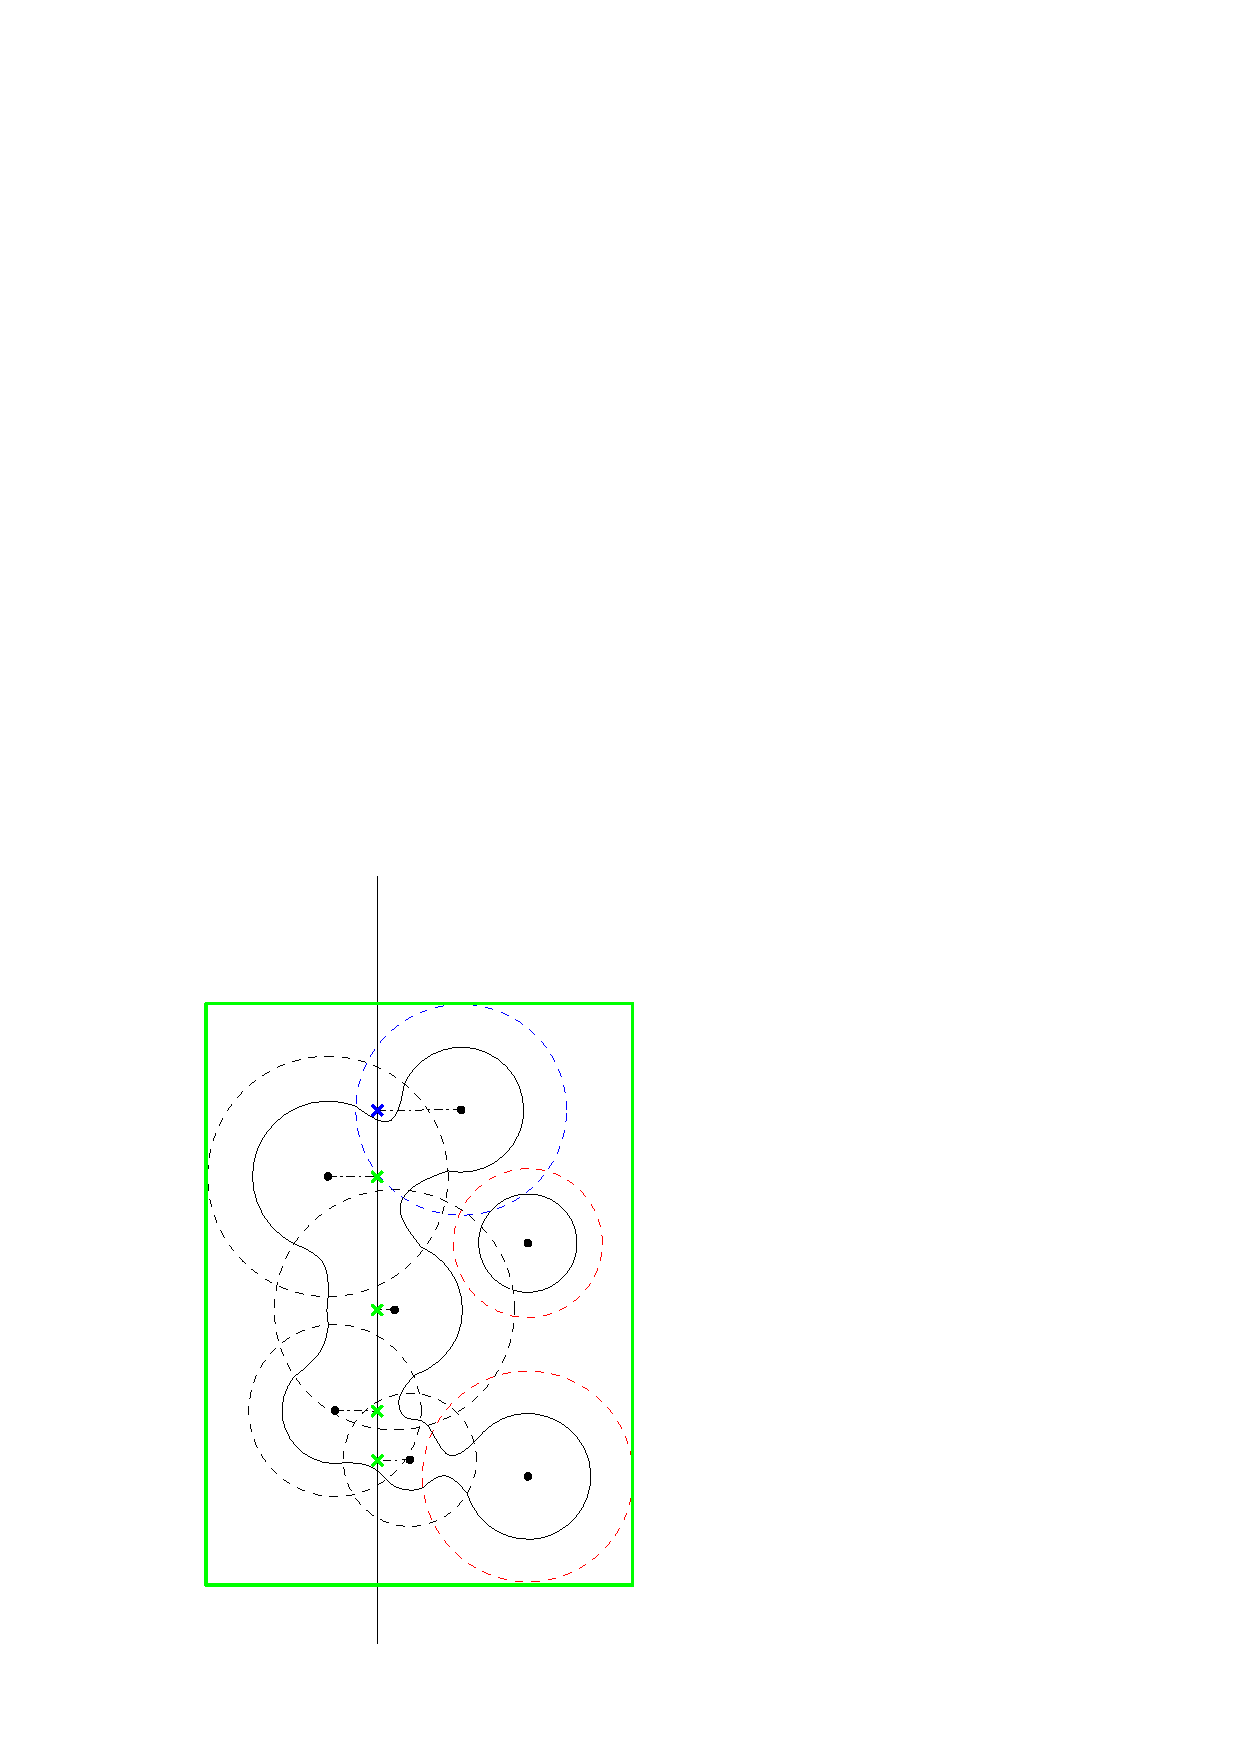
\includegraphics[width=1.5in]{../../figs/bisect1.pdf}}
  \subfloat[][]{\label{bis2}\includegraphics[width=1.5in]{../../figs/bisect2.pdf}} 
  \caption{Illustration of the ray-surface intersection algorithm.}
  \label{bisection}
\end{figure}

\subsubsection{Limitations}

With this technique we can track the surface efficiently but some ray-intersection are missed.
This is the case when two primitives are just close enough to start blending. Figure \ref{miss} illustrates an example of a ray that miss the surface.

Our method to find a point inside the surface with a line segment primitive also causes artefacts when the direction oh the view is close to being parallel to the segment's axis.

\begin{figure}[ht]
  \centering
  \includegraphics[width=2.0in]{../../figs/miss.pdf}
    \caption{Example of a ray that miss the surface with our intersection method.}
  \label{miss}
\end{figure}



\subsection{Evaluation of the method}

Our algorithm allows to render our skeletal implicit surfaces at interactive frame rate.
The root finding by bisection is fast and easy to implement. The surface is found in less than 10 bisection steps for a precision that doesn't  present visible artefacts.
However, selecting the primitives that have an influence on the ray requires to evaluate the entire function for each primitive which leads to a $n^2$ complexity. This does not scale very well for large models. A solution would be to use a bounding volume hierarchy as presented in \cite{Gourmel-2010-FBVH}. However, constructing such a BVH at every frame is expensive and traversing the hierarchy on the GPU has a non negligible cost.

Ray-tracing the surface remains very slow in comparison to rendering the tessellated mesh, our models are rendered at 20 to 100 fps depending on the complexity of the models against around 2000 fps for the tessellated meshes on an NVidia Quatro FX 5800.

It is also worth mentioning that the algorithm is very sensitive to the area on the screen covered by the surface since most of the rendering computations are done on the fragment shader. This is interesting because the cost of rendering the model is resolution dependant rather than geometry dependant. To provide a more scalable level of detail technique, it could be interesting to discard primitives that are too small to produce visible details.


\section{Rigging and Animation}

To animate the surface, we simply update the positions of the primitives in the CPU. This can be done easily by attaching them to a hierarchical skeleton data structure.

We investigated two different work-flows to produce rigged and animated surfaces.
The first approach is very similar to the rigging process used with polygonal models. It consists in modelling the surface with metaballs and metatubes in a first time. Then the modeller creates a rig for the surface and finally the primitives are attached to the rig.

This work-flow with our modelling tool is illustrated in figure \ref{workflow1}.
From the left to the right : the model is sculpted with metaballs, a rig is positioned on the model, primitives are selected and attached to a specific bone, the surface is ready to be animated and we can create poses by orienting the bones.

\begin{figure}[ht]
  \centering
  \includegraphics[width=3.5in]{../../figs/workflow1.png}
  \caption{Work flow with metaball sculpting.}
  \label{workflow1}
\end{figure}

Since we use line  segment primitives in our surface representation, the segments are natural candidates to provide the bone structure.

With this in mind, we developed another work-flow.
We start by creating the armature of the model but the bones are used as primitives for the implicit surface.
Then, the radius of these primitives are adjusted to give the right silhouette to the model. Finally we can add details with metaballs and attach them to the bones.

Figure \ref{workflow2} illustrates how we model a dinosaur with this work-flow.
From the left to the right :  the skeleton is created with tube primitives attached to the bones, the surface is edited by modifying the radius of the metatubes and by adding a few metaballs for the head and the feet and the surface is ready to be animated.

\begin{figure}[ht]
  \centering
  \includegraphics[width=3.5in]{../../figs/workflow2.png}
  \caption{Work flow with skeletal implicit surfaces.}
  \label{workflow2}
\end{figure}


\section{Texturing}


Texturing implicit surfaces is not straightforward because we don't have access directly to points on the surface so we cannot attach texture coordinates as we would do with a triangle mesh.

A common approach to tackle this problem is to use hyper textures or 3D textures to cover the space in which the surface is embedded and simply looking up the texture with the fragment's position.

Another approach is to use texture projectors to generate the texture coordinated for a 2D texture mapping.
For example, an implicit surface generated by a line segment can be intuitively textured using a cylindrical projection.
When we draw a fragment on this surface, we compute its cylindrical coordinates in the referential of the line segment and use these as texture coordinates.


Figure \ref{tubetex} shows a simple tube surface textured with a cylindrical projection. 
\begin{figure}[ht]
  \centering
  \includegraphics[width=1.5in]{../../figs/TubeTextured.png}
  \caption{A simple tube surface texture mapped with a cylindrical projection.}
  \label{tubetex}
\end{figure}

It is possible to use other kind of projections such as spherical or planar.

Wyvill et al. proposed a more advanced scheme in \cite{Tigges98texturemapping}to texture skeletal implicit surfaces by shooting particles from the surface to a well parametrized support surface using the gradient of the field.
This method allow less distortion in the mapping than simple projections but problems still occurs at the intersection of primitives and computing the trajectories of the particles for each fragment is prohibitive for a real time ray-tracer.


\subsection{Surface skinning}

Using local texture projections and computing the texture coordinates on the fragment shader allow to apply texture to our surfaces with user control.

However, with animation, having a coherent texture mapping requires to animate the projectors as well as the model.
Also, having a projector for each primitive is not adapted for regions where several primitives have an influence.
One could blend the different textures but this gives poor results.

To address this issue, we propose a method that is inspired by vertex skinning.

The method consists in texturing the model in a rest position using local texture projectors.
The designer can use an arbitrary number of projectors with different projections.

Then, when rendering the animated model, we assign bone weights to the fragment depending on it's distance to the bones and we use them to transform the fragment's position to the rest pose space. Then we compute the texture coordinates of the fragment by using the local projectors and look up the texture accordingly.

Figure \ref{weightSkin} shows an example of how the textures are applied. The model is composed of two segment primitives associated to bones and textured by a single cylindrical projector. On the left, the colours show the weights of the fragments associated with the two bones. On the right, we see that the texture mapping follows the deformation of the surface.

\begin{figure}[ht]
  \centering
  \includegraphics[width=1.5in]{../../figs/skintexture.png}
  \caption{Illustration of the skinning scheme used for texturing.}
  \label{weightSkin}
\end{figure}

Listing \ref{skinning} shows the pseudo code for this technique.

\begin{algorithm}                      % enter the algorithm environment
\caption{Transformation of the vertex positions for texturing}          % give the algorithm a caption
\label{skinning}                           % and a label for \ref{} commands later in the document
\begin{minipage}{0.9\textwidth}%
\CPP

vec3 pointOnSurface;
vec3 restPosition = vec3(0,0,0);	

for(int bone = 0; bone <  nbBones; bone++)
{
	//compute fragment weight wtrt. the bone
	float w = weight(bone, pointOnSurface);
	//transform
	vec3 transformed = pointOnSurface;
	//Back to object space
	transformed += boneInvTrans[bone][3].xyz;
	transformed = boneInvTrans[bone]*transformed;
	//to rest world space
	transformed = boneRestTrans[bone]*transformed;
	transformed.xyz += boneRestTrans[bone][3].xyz;
	//sum
	restPosition += w*transformed.xyz;;
}

//Compute the texture coordinates of the fragment in rest position
vec2 uv = texCoord(restPosition);

\END\PROGd{}

\end{minipage}%
\end{algorithm}


This method showed good results and is adaptable for 3D textures as shown in figure \ref{skinsequence}. To implement this technique, we send to the GPU the transformation matrices of the bone in rest position as well as the inverse of the bone's current transformation matrices. The computation to find the position of the fragment in rest position are negligible in comparison to the ray tracing of the surface. We implemented this method as a proof of concept but giving the control on the radius of influence of the bones can lead to more robust implementations. Also, using this technique as well as using local texture projectors implies that we have to search for the bones and projectors that have an influence on a point of the surface.

\begin{figure}[ht]
  \centering
  \includegraphics[width=3.5in]{../../figs/Sequences.png}
  \caption{Illustration of the skinning scheme used for texturing.}
  \label{skinsequence}
\end{figure}

\subsection{Displacement mapping}

To enhance details on the surface, techniques such as normal mapping and displacement mapping are commonly used in computer graphics.
To apply these effects with a polygonal representation, we need to provide a texture mapping and the tangent vector to the surface.

With implicit surfaces, we can add a value to the field function to add relief details.
Also, because the normal is computed from the gradient of the field function, the perturbation is applied automatically to the surface normal.

In this way, if the perturbation is small enough to keep the function null outside the support of the original function, we can apply the displacement while the ray-surface intersection is searched.

This method applies very easily with hyper-textures as shown on figure \ref{hyperdisp}.
It can also be applied with projected 2D  as shown on figure \ref{disp} but the uv coordinates have to be computed at each step of the intersection search.

\begin{figure}[ht]
  \centering
  \includegraphics[width=2.0in]{../../figs/TubeDispNoise.png}
  \caption{Displacement mapping with a 3D noise function.}
  \label{hyperdisp}
\end{figure}

\begin{figure}[ht]
  \centering
  \includegraphics[width=2.0in]{../../figs/TubeDisp.png}
  \caption{Displacement mapping with a projected 2D texture.}
  \label{disp}
\end{figure}

This method is not robust enough when using our optimization with bisection because the point inside the surface computed as described in section \ref{bisectsec} is no longer guaranteed to be inside the surface. Also with sharp derails there might be more than one intersection on the ray between our initial point and the outside.

For animated surfaces the method cannot be applied either.


\section{Results and discussions}


We revisited geometric modelling with implicit surfaces. We used a simple surface representation with skeletal implicit surfaces that allowed to model quickly interesting models.
We implemented a real time renderer based on ray-tracing adapted for our surface representation. This method allows to render at interactive frame rate animated models. Although this method is far from being as efficient as polygon rendering, it has some advantages such as it's simplicity, the compactness of the models representation and a very small amount of memory to send to the GPU to render smooth surfaces.

We investigated the possibilities to allow texturing with user control and developed a method to keep a coherent texture mapping during animation.

We showed the possibilities to integrate displacement mapping in the rendering but this method is limited to static models and can't benefits of the speed up provided by the bisection algorithm. 

In conclusion, using implicit surfaces for the surface representation and ray-tracing for the rendering seems to be an alternative to polygon rendering that provides simplicity as well as flexibility. The main issue that remains is efficiency. Using the current graphics architecture and our method, using implicit surfaces to render models is prohibited in commercial applications where the scene includes a great number of models.

However, it is likely that better ray-tracing algorithm and future advances of the graphics hardware can provide better performances with the same advantages. We have mentioned for example sphere tracing, B\'ezier clipping and the use of bounding volume hierarchies.

In future works, it would be interesting to investigate the possibility to implement a real time ray-tracer for a wider range of skeletal surfaces. For example, it would be interesting to use convolution surfaces with primitives such as parametric curves. It would also be interesting to implement a real time ray-tracer for the Blob-Tree, thus providing a renderer for sketch-based modelling tools.



\bibliographystyle{acmsiggraph}
\bibliography{../references}
\end{document}
